\documentclass[11pt]{article}
\usepackage[margin=1in]{geometry}
\usepackage{amsmath,amssymb,amsthm}
\usepackage{booktabs}
\usepackage{array}
\usepackage{microtype}
\usepackage{siunitx}
\usepackage{tikz}
\usepackage{algorithm}
\usepackage[noend]{algpseudocode}
\usepackage[hidelinks]{hyperref}
\usepackage[capitalise]{cleveref}

\newtheorem{proposition}{Proposition}
\newtheorem{lemma}{Lemma}

\sisetup{detect-all}
\newcommand{\us}{\,\si{\micro\second}}

\title{Fewer, Better Guesses: A Scalar Band Solver\\that Outperforms SIMD Sudoku Solvers on Apple Silicon}
\author{James Kelly}
\date{September 2026}

\begin{document}
\maketitle

\begin{center}
\begin{minipage}{0.85\textwidth}
\small\textbf{AI use.} This work was done depending heavily on Anthropic's LLM harness Claude (Claude Code), using the model Claude Opus~5.5 with occasional advisory support from Claude Fable, including in theorizing, experimentation, and writeup.
\end{minipage}
\end{center}


\begin{abstract}
The fastest published solver for hard Sudoku puzzles, tdoku, combines a SIMD encoding of the grid with strong propagation, and on x86 its author's benchmark shows it well ahead of the other fast solvers on hard puzzles. We ported tdoku to ARM NEON and
found that on Apple Silicon its lead over scalar solvers shrinks, but it still wins on the hardest puzzles. We then
built FastBandSolver, a scalar solver on the band representation of zhouyundong and JCZSolve (a band is a row of
three boxes; the representation stores each digit's candidates per band as a bit mask), and made three changes:
(1) a \emph{stack rule} that prunes each digit's columns within each column of three boxes, keeping only choices that
fit a one-to-one pairing of bands with columns (a perfect matching), which generalizes locked candidates; (2) branching on the two-candidate cell with the most unsolved peers instead of the first one found;
(3) a fewest-candidates fallback when no two-candidate cell exists. On an Apple M4 Max, checking uniqueness (a
solution limit of 2) as in tdoku's benchmarks, FastBandSolver is 1.08--1.62$\times$ faster than native tdoku on all
five of tdoku's standard data sets, including 1.20$\times$ on the 375 hardest forum puzzles. An ablation attributes
the gain mainly to branching: the search makes 138 guesses per puzzle on that set where JCZSolve makes 363. Compared with tdoku's published x86 results, scalar solvers gain much more from the M4 than tdoku does, and a
projection suggests FastBandSolver would be about 0.7 times tdoku's speed on a recent Intel processor with AVX-512:
the advantage is specific to Apple Silicon. We also report five approaches that did not beat tdoku, with measurements: template (pattern-overlay) search, several
search-tree nodes in SIMD lanes, lookahead probing, triad rules, and joining band fillings.
\end{abstract}

\section{Introduction}

Solving a single Sudoku is easy for a computer, but solving and \emph{proving uniqueness} of millions of hard
puzzles quickly matters to puzzle generators, to difficulty raters and to exhaustive searches such as the proof
that no 16-clue Sudoku exists~\cite{mcguire2014sixteen}. Deciding whether a partial Latin-square-like puzzle has another
solution is NP-complete~\cite{yato2003complexity}, so every fast solver is a search with propagation, and the design space is
the classic one of constraint programming~\cite{simonis2005sudoku} and SAT~\cite{lynce2006sudoku}: how much inference to do at
each node, and where to branch.

The current reference point is tdoku~\cite{dillon2019tdoku,dillon2019nerdsniped}. It encodes the grid in 128- or
256-bit SIMD registers, reasons about \emph{triads} (the three cells of a row or column within a box) in both
orientations, and in its author's benchmark it is well ahead of the other fast solvers on hard puzzles, though slower than two of them on the easiest ones (\cref{sec:related}). tdoku targets x86 SSE and AVX; to compare on ARM, we added native NEON support
to it~\cite{kelly2026tdokuarm}. On Apple Silicon the picture changes (\cref{sec:arm}): scalar solvers run much faster than on x86, while tdoku does not, and the scalar band solver JCZSolve~\cite{jczsolve2016} already beats tdoku on the
17-clue set, but tdoku keeps its lead on the hardest puzzles.

This paper asks whether a scalar solver can beat tdoku on the hard sets too, and answers yes. \Cref{sec:terms}
explains the background for readers new to the area: the parts of the grid, propagation and search, bitmasks, and
perfect matchings. Our contributions:

\begin{itemize}
\item \textbf{FastBandSolver}, an open-source C++ solver (\cref{sec:solver}) that is faster than native tdoku on all
  five of tdoku's standard data sets on an Apple M4 Max (\cref{tab:sota}).
\item A \textbf{stack rule} (\cref{sec:rules}): each digit's use of columns within a stack is a perfect matching
  of bands to columns, and pruning edges that lie on no perfect matching subsumes locked candidates. Together with
  the familiar band rule, it makes box and column hidden singles redundant on these data sets.
\item An \textbf{ablation}, switching each of our changes off in turn, (\cref{tab:ablation}) showing that branching, not propagation, carries most of the gain:
  picking the two-candidate cell with the most unsolved peers cuts the tree by 45\% at almost no cost, and a
  fewest-candidates fallback removes another 12\% of the time on the hardest set, even though it fires at only 1\%
  of branch nodes.
\item \textbf{Negative results} with measurements (\cref{sec:negative}): complete per-digit template inference,
  running search-tree nodes in SIMD lanes, lookahead, triad rules, and band decomposition all fail to beat tdoku
  here, and we say why.
\end{itemize}

\section{Background: how fast Sudoku solvers work}
\label{sec:terms}

This section explains the ideas the rest of the paper relies on, for readers who know some programming but not the
Sudoku-solving literature. Readers who know it can skip to \cref{sec:related}.

\subsection{The puzzle and its parts}

A Sudoku grid has 81 \emph{cells} arranged in 9 \emph{rows} and 9 \emph{columns}, and divided into 9 \emph{boxes}, the
$3\times 3$ blocks outlined in \cref{fig:grid}. Rows, columns and boxes are together called \emph{units}. A puzzle
fills in some cells, the \emph{clues}, and the goal is to fill in the rest so that each digit 1--9 appears exactly
once in every unit. A well-formed puzzle has exactly one solution. The \emph{peers} of a cell are the 20 other cells
that share a row, column or box with it; a cell's digit can never appear in any of its peers.

Two larger structures matter in this paper. A \emph{band} is a horizontal strip of three boxes: rows 1--3, 4--6 or
7--9, 27 cells in all. A \emph{stack} is a vertical strip of three boxes: columns 1--3, 4--6 or 7--9. There are three
bands and three stacks, and each box is where one band and one stack cross. Within a band, the three cells where a row
crosses a box form a \emph{mini-row}, so each band has nine mini-rows; within a stack, the three cells where a column
crosses a box form a \emph{mini-column}. Mini-rows and mini-columns are what tdoku's author calls \emph{triads}. When
we look inside a single band we number its rows and its boxes 0--2 and its columns 0--8.

\begin{figure}[t]
\centering
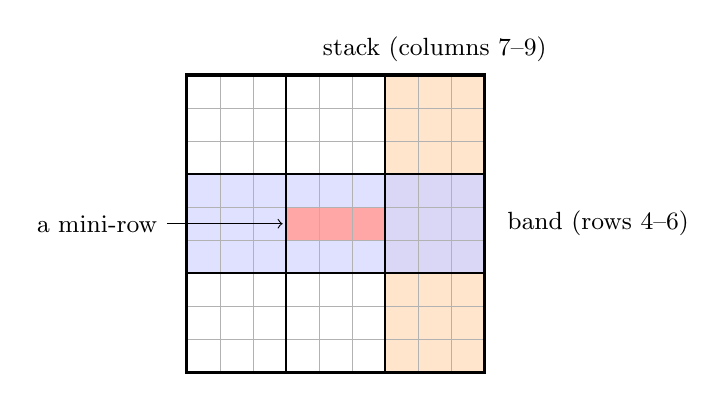
\begin{tikzpicture}[x=0.42cm,y=0.42cm]
  \fill[blue!12] (0,3) rectangle (9,6);          % a band (the middle one)
  \fill[orange!20] (6,0) rectangle (9,9);        % a stack (the right one)
  \fill[orange!20!blue!18] (6,3) rectangle (9,6);% their shared box
  \fill[red!35] (3,4) rectangle (6,5);           % a mini-row
  \draw[step=1,gray!60,very thin] (0,0) grid (9,9);
  \draw[very thick] (0,0) rectangle (9,9);
  \foreach \x in {3,6} { \draw[thick] (\x,0) -- (\x,9); \draw[thick] (0,\x) -- (9,\x); }
  \node[right] at (9.4,4.5) {\small band (rows 4--6)};
  \node[above] at (7.5,9.1) {\small stack (columns 7--9)};
  \draw[->] (-0.6,4.5) node[left] {\small a mini-row} -- (2.9,4.5);
\end{tikzpicture}
\caption{The parts of a Sudoku grid used in this paper. The shaded horizontal strip is a band, the shaded vertical
strip is a stack, and their overlap is a box. The dark cells are a mini-row: the three cells where a row of the band
crosses one of its boxes.}
\label{fig:grid}
\end{figure}

\subsection{Candidates and propagation}

A solver keeps, for every empty cell, the set of digits that could still go there: its \emph{candidates}. At the start a
cell's candidates are the digits not already used by a clue among its peers. Solving then alternates between two
activities. \emph{Propagation} applies logical rules that remove candidates which cannot be part of any solution, and
\emph{search} makes a guess when the rules run out.

The simplest rules are the ones human solvers learn first:
\begin{itemize}
\item A \emph{naked single} is a cell with only one candidate left: that digit must go there.
\item A \emph{hidden single} is a digit that has only one possible cell left in some unit. For example, if in row 5
  the digit 7 is a candidate in only one cell, then 7 goes there, even if that cell has other candidates too. When the
  unit is a row we call it a \emph{row single}.
\item \emph{Locked candidates} use the overlap between a box and a row or column. For example, if every candidate for 3
  in the top-left box lies in column 2, then the 3 of that box must be in column 2, so 3 can be removed from column 2
  in the other two boxes of the stack.
\end{itemize}
Placing a digit removes it from all the cell's peers, which can create new singles, so rules are applied repeatedly
until nothing changes. That state is called a \emph{fixed point}. Human solvers know many more rules (pairs, X-wings,
chains and so on); fast computer solvers use only a few cheap ones and search for the rest.

\subsection{Search, guesses and uniqueness}

When propagation stops but cells are still empty, the solver picks a cell and tries its candidates one at a time.
Each try copies the current state, places the digit, and propagates again; if that leads to a cell with no candidates,
the try is a dead end and the solver \emph{backtracks} to the next candidate. This is depth-first search. Its tries
form a \emph{search tree}: each \emph{node} is a state after propagation, and each branch is a guess. We count a cell
with two candidates as one \emph{guess} (one binary decision) and a cell with $n$ candidates as $n-1$.

The benchmark used throughout this paper asks each solver to find up to two solutions (a \emph{solution limit} of 2).
Finding one solution shows the puzzle is solvable; failing to find a second one proves it is \emph{unique}. For a
well-formed puzzle that means the solver cannot stop at the first solution: it must rule out every other branch of the
tree. So the total time is roughly
\[
\text{time} \approx (\text{nodes in the search tree}) \times (\text{time per node}).
\]
Stronger rules make the tree smaller but each node slower; cheaper rules do the opposite. The choice of \emph{which}
cell to guess on also changes the size of the tree, sometimes by a large factor, at little cost per node. This
trade-off is the subject of the paper.

\subsection{Sets as bits}

Fast solvers do not store candidates as lists. They store a set of up to 32 small numbers as the bits of one 32-bit
integer, a \emph{bitmask}: bit $i$ is 1 when $i$ is in the set. Set operations then become single processor
instructions: intersection is bitwise AND ($\&$), union is OR ($\mid$), removing elements is AND with the complement
($\lnot$), and shifting the bits left or right ($\ll$, $\gg$) moves every element by the same amount at once. The
\emph{popcount} instruction counts the 1-bits, which is the size of the set. For example, the set $\{0, 2, 3\}$ is the
bitmask $1101_2 = 13$, and ANDing it with $\{2,3,4\} = 11100_2$ gives $\{2,3\} = 1100_2$ in one instruction.

We write bitmasks in \emph{octal} (base 8), marked with a subscript 8, because one octal digit is exactly three bits,
and Sudoku is built from threes. For example $7_8 = 111_2$ is three 1-bits, $777_8 = 111\,111\,111_2 = 511$ is nine,
the mask of all nine columns of one row, and $410005022_8$ is a 27-bit mask whose nine octal digits are the nine
mini-rows of a band (\cref{sec:state}).

A \emph{lookup table} is a precomputed array: instead of computing a function of a small input at run time, the solver
reads the answer from memory, indexed by the input. A 9-bit input has only $2^9 = 512$ possible values, so any function
of 9 bits can be tabulated in a 512-entry array. The solvers in this paper rely heavily on such tables.

\subsection{What makes code fast on a modern processor}

A modern processor core executes several instructions per clock cycle, as long as they do not depend on each other.
The number actually achieved is the \emph{IPC} (instructions per cycle). Two things lower it in search code.
\emph{Branch mispredictions}: the processor guesses the outcome of each \texttt{if} ahead of time, and a wrong guess
discards the work done after it; search code has many data-dependent branches. \emph{Dependency chains}: an
instruction that needs the result of the previous one has to wait for it. \emph{SIMD} (single instruction, multiple
data) instructions operate on a wide register holding several small values at once, for example eight 16-bit numbers
in a 128-bit register. x86 processors offer 128-bit (SSE) and 256-bit (AVX2) SIMD; ARM processors such as Apple's
offer 128-bit SIMD called NEON. A solver whose data fits a SIMD register can process a whole box or band in a few
instructions; a \emph{scalar} solver uses ordinary 32- or 64-bit integers.

\subsection{Matchings}

The rules at the heart of this paper are phrased in terms of matchings, a basic notion from graph theory. A
\emph{bipartite graph} has two sets of vertices, for example the three rows and the three boxes of a band, and edges
that each join one vertex of the first set to one of the second. We draw a row--box edge when a digit still has a
candidate in that row's mini-row in that box. We can write such a graph as a $3\times 3$ table of 0s and 1s, its
\emph{biadjacency matrix} $A$, with $A_{ij}=1$ when vertex $i$ of the first set and vertex $j$ of the second are joined.

A \emph{matching} is a set of edges no two of which share a vertex. A \emph{perfect matching} uses every vertex exactly
once; with three vertices on each side it is a one-to-one pairing of the two sets, that is, a choice of three 1-entries
of $A$ with one in each row and one in each column of the table. There are at most $3! = 6$ of them. An edge \emph{lies
on a perfect matching} when at least one perfect matching includes it. Why this matters: a digit appears once in each
row of a band and once in each box of the band, so its final placement pairs the three rows one-to-one with the three
boxes, which is exactly a perfect matching. Any row--box edge that lies on no perfect matching can therefore never be
used, and the digit can be removed from that mini-row. In \cref{fig:band}, row 1 can only use box 0; that forces row 0
into box 1 and row 2 into box 2, so the only perfect matching is row 0--box 1, row 1--box 0, row 2--box 2, and the two
other edges can be removed.

Hall's theorem~\cite{hall1935representatives} says exactly when a perfect matching exists: every set of $k$ vertices on
one side must be joined to at least $k$ vertices on the other. Many human solving techniques are special cases of this
idea. We also use the \emph{permanent} of a $2\times 2$ matrix $\bigl(\begin{smallmatrix} a & b \\ c & d
\end{smallmatrix}\bigr)$, which is $ad+bc$ (the determinant with a plus sign); for a 0-1 matrix it is nonzero exactly
when the two-by-two graph has a perfect matching.

Finally, a \emph{template} is one complete way of placing a single digit nine times, once in every row, column and
box. There are 46{,}656 templates; \cref{sec:negative} tests a solver built on them.

\section{Related work}
\label{sec:related}
\label{sec:background}

Sudoku has been attacked with every general-purpose search technique, and a community of hobbyist programmers,
largely on the Sudoku Players' Forum, has spent two decades making special-purpose solvers fast. This section
describes what the solvers we build on and compare with actually do, from their source code and their authors'
write-ups, and then says exactly what we took from each.

\subsection{Three general encodings}

\paragraph{Exact cover.} A Sudoku is an \emph{exact cover} problem: there are 729 possible choices (a digit in a
cell) and 324 constraints (each cell filled once, and each digit once in each row, column and box), and a solution is a
set of 81 choices that satisfies every constraint exactly once. Knuth's \emph{dancing links} algorithm (Algorithm X
with a linked-list representation) solves exact cover problems and discusses Sudoku at length in
\emph{The Art of Computer Programming}~\cite{knuth2022taocp4b}. kudoku~\cite{attractivechaos2011kudoku}, the fastest
exact-cover solver in tdoku's benchmark, uses this formulation without dancing links: it stores for each choice its 4
constraints and for each constraint its 9 choices, keeps a count of the remaining choices per constraint, always
branches on the constraint with the fewest remaining choices, and undoes a branch by reversing the counts rather than
copying the state. Its source describes it as a faster version of Stertenbrink's \texttt{suexco.c}. In this
formulation naked and hidden singles happen automatically (a constraint with one choice left), but locked candidates
do not.

\paragraph{SAT.} Lynce and Ouaknine~\cite{lynce2006sudoku} encoded Sudoku as a Boolean satisfiability problem, with
a variable for each (cell, digit) pair and clauses saying each cell has a digit and no unit has a digit twice, and related SAT propagation techniques to human solving techniques. The standard SAT algorithm DPLL
alternates \emph{unit propagation} (a clause with one literal left forces it) with branching.

\paragraph{Constraint programming.} Simonis~\cite{simonis2005sudoku} modelled Sudoku with \texttt{alldifferent}
constraints, one per unit, and compared how strongly different propagation methods filter them. The strongest
standard method is R\'egin's algorithm~\cite{regin1994filtering}, which models an \texttt{alldifferent} constraint as a
bipartite graph between variables and values and removes exactly the edges that lie on no matching covering every variable (a perfect matching, when there are as many values as variables). Our band
and stack rules apply the same principle to a much smaller graph, three rows or bands against three boxes or
columns, which is small enough to precompute every case in a table.

\subsection{Fast cell-based solvers}

\paragraph{Norvig.} Norvig's widely read 2006 essay~\cite{norvig2006sudoku} stores the candidates of each cell as a
string of digits in a dictionary, and uses two rules: if a cell has one candidate, remove it from its peers (naked
singles); if a unit has one place for a digit, put it there (hidden singles). It searches depth first, choosing the
cell with the fewest candidates, the \emph{minimum remaining values} heuristic of Haralick and
Elliott~\cite{haralick1980increasing}, and copies the whole state at each guess. It is written for clarity, not speed.

\paragraph{JSolve.} Linhart's JSolve~\cite{linhart2010jsolve}, which tdoku's documentation traces back to the earlier
bb\_sudoku, keeps a 9-bit candidate mask per cell and a mask of placed digits per unit. It propagates naked singles
through a queue of pending placements, finds hidden singles with bitwise ``seen once / seen more than once'' masks per
unit, and applies locked candidates to groups of three-cell strips. It guesses on the cell with the fewest candidates,
stopping its scan as soon as it finds a cell with two, and saves the board on a stack to undo a guess.

\paragraph{FSSS and fsss2.} Dobrichev's FSSS (2010) is a cell-based solver of the same kind. fsss2~\cite{dobrichev2014fsss2}
(2014) switches to a per-digit layout: for each digit, one 128-bit word whose bits 0--80 mark the cells where the
digit is possible and whose upper bits mark the units where it is not yet placed. Naked singles are found by counting,
across the nine digit words, how many digits each cell admits, using bit-parallel adders that process all 81 cells at
once; hidden singles by checking each unsolved unit for a single bit; and locked candidates and naked pairs are
compile-time options. By default it guesses on a cell with the fewest candidates, taking the lowest digit and the
leftmost cell. Its source also contains experimental alternative guess strategies, switched off by default, including
choosing by the number of direct eliminations; a comment notes one of them as slower than another alternative.

\subsection{Band solvers: zhouyundong, JCZSolve and rust\_sudoku}

In 2012 the forum user zhouyundong\_2012 posted a solver~\cite{zhouyundong2012solver} built on a different layout,
which we call the \emph{band representation}: one 32-bit word per (digit, band), whose 27 low bits mark the cells of the
band where the digit is still possible. The forum members champagne and JasonLion refined it into
JCZSolve~\cite{jczsolve2016}, whose header credits zhouyundong with ``storing bands by digit and the Update routine'',
and champagne with ``the pairing of ApplySingleOrEmptyCells and GuessBiValueInCell''. Emerentius ported it to
Rust~\cite{emerentius2018sudoku}. Because FastBandSolver starts from this design, we describe JCZSolve in detail.

\paragraph{Update.} For each (digit, band) word that changed since the last pass, JCZSolve does the following with
512-entry lookup tables. It compresses each 9-bit row into the 3 boxes the digit can still use in that row, giving a
$3\times 3$ row-by-box pattern for the band. A second table keeps only the parts of that pattern that some valid
assignment of rows to boxes can use, and returns zero, a contradiction, if there is none. This is the band rule of
\cref{sec:rules}, though the source does not describe it in terms of matchings. A third table, indexed by the columns
the digit still uses in the band, removes from the other two bands every column that is the only column left in one
of this band's boxes: locked candidates from a box into a column. Further tables detect rows that are down to one
cell, and those cells are removed from the other eight digits' words. Emerentius notes that over 80\% of the solver's
time is spent in this routine.

\paragraph{Singles and guessing.} After the updates, \texttt{ApplySingleOrEmptyCells} counts, for each band, how many
digits each cell admits, with three 27-bit words meaning ``at least one'', ``at least two'' and ``at least three''
(the same trick as fsss2's adders, on one band at a time). Cells with none are a contradiction, cells with one are
placed, and cells with exactly two are saved, so the next step, \texttt{GuessBiValueInCell}, has a list of
two-candidate cells for free. It guesses on the first of them in board order, copying the state into the next slot of
a fixed array. If there is none, \texttt{GuessFirstCell} tries every candidate of the first unsolved cell; its
comment reads ``Kind of dumb, but \_way\_ fast code''. rust\_sudoku keeps this design, removes one hard-to-predict
branch, and when there is no two-candidate cell checks up to three cells and guesses the one with the fewest
candidates.

\subsection{tdoku}

Dillon's tdoku~\cite{dillon2019tdoku,dillon2019nerdsniped} approaches Sudoku as a SAT problem and then specializes the
SAT machinery until it fits in SIMD registers. His write-up is a careful study of the design space, and we follow its
benchmark methodology.

\paragraph{From DPLL to triads.} The write-up starts from DPLL with a variable per (cell, digit), adds clauses saying
that each row, column and box contains each digit, so that hidden singles follow from unit propagation, and observes
that locked candidates are exactly the deductions this still misses. To capture them it adds new variables for the
triads, the mini-rows and mini-columns: a triad variable for digit $v$ is true when $v$ is in that triad. Rows,
columns and boxes then become ``exactly one of these three triads'' constraints, and each triad must contain exactly
three digits. All of these are cardinality constraints, applied by one rule: when the number of literals still possible
equals the number required, all of them are asserted.

\paragraph{Band configurations.} For one digit, the nine triads of a band can only be true in six patterns, one per
assignment of the band's rows to its boxes; the write-up calls these \emph{configurations}. tdoku stores, for each band
(horizontal and vertical) and each of its six configurations, the 9-bit set of digits that can still take it. The
write-up notes that configurations add no new deductions, but ``do in one step what previously might have required
multiple steps''. The six configurations of a band are the six perfect matchings of \cref{sec:terms}, so tdoku's band
state is our band rule in a different form, maintained for rows and columns alike.

\paragraph{SIMD layout and propagation.} Each box is one 256-bit register viewed as a $4\times 4$ matrix of 16-bit
lanes: the $3\times 3$ part holds the candidate sets of the box's nine cells, and the extra row and column hold the box's triad variables. Propagation is message passing: a box sends eliminations to its horizontal and vertical bands, and a band
turns its remaining configurations back into allowed triads and restricts its three boxes. Every step is branch-free
SIMD code. On x86 without AVX2, and on our ARM port, each 256-bit value is a pair of 128-bit registers.

\paragraph{Branching.} tdoku picks the band, horizontal or vertical, with the fewest remaining configurations over all
digits, and in it a digit with the fewest configurations (two if possible), and branches on keeping or removing one
configuration. It copies the whole state for the first branch and reuses the original for the second.

\paragraph{Reported results.} On an Intel i5-8600k, with a solution limit of 2 as here, the write-up reports tdoku at
about 1.5 times the geometric mean speed of the other solvers on magictour and approaching twice on the hardest set,
with 113 guesses per puzzle on that set against 15 to 367 for the others, and notes that it is slower than fsss2 and
sk\_bforce2 (by GPenet, 2018) on the easiest puzzles. The write-up also reports an experiment that bears directly on
this paper: adding strongly-connected-component analysis of the implication graph cut the guesses on magictour to 3.35
per puzzle, but every variant was slower, and the author chose ``to focus on being fast''.

\paragraph{Counting guesses.} Guess counts are not comparable across solvers without care. tdoku counts one per branch
point; JCZSolve counts one per two-candidate branch but one per digit tried in its fallback; kudoku counts only
branches with more than one choice. We count one per two-candidate branch and $n-1$ for an $n$-candidate cell.

\subsection{Branching heuristics, lookahead and structure}

Choosing the variable with the fewest remaining values~\cite{haralick1980increasing} is the classic heuristic, and
most Sudoku solvers use a version of it; the band solvers use the cheaper ``first two-candidate cell''. Lookahead
SAT solvers~\cite{heule2009lookahead}, and Algorithm L in Knuth's treatment of satisfiability~\cite{knuth2022taocp4b},
choose a branch by tentatively propagating candidate decisions and scoring the result, and treat a decision whose
propagation fails as a free deduction. St\aa lmarck's method~\cite{sheeran2000tutorial} goes further and keeps the
conclusions that both branches of a split share. We test lookahead in \cref{sec:negative}.

Felgenhauer and Jarvis~\cite{felgenhauer2006mathematics} counted all Sudoku grids by enumerating the fillings of the
top band and extending them, and McGuire, Tugemann and Civario~\cite{mcguire2014sixteen} proved by an exhaustive computer search that no puzzle with 16 clues has a unique solution. Yato and
Seta~\cite{yato2003complexity} showed that deciding whether a puzzle has another solution besides a given one is
NP-complete, so no fast solver can avoid search in general. Human solvers use the \emph{pattern overlay} or template
method, credited to Myth Jellies~\cite{stuart2008pom}, which tests each digit's placement against all 46{,}656
templates; we test it as a solver in \cref{sec:negative}.

\subsection{How this work builds on prior work}

\Cref{tab:lineage} summarizes where each part of FastBandSolver comes from.

\begin{table}[t]
\centering
\caption{Where each part of FastBandSolver comes from.}
\label{tab:lineage}
\small
\renewcommand{\arraystretch}{1.25}
\begin{tabular}{>{\raggedright\arraybackslash}p{3.3cm}>{\raggedright\arraybackslash}p{4.6cm}>{\raggedright\arraybackslash}p{6.0cm}}
\toprule
part & taken from & what we changed \\
\midrule
27-bit mask per (digit, band) & zhouyundong~\cite{zhouyundong2012solver}, JCZSolve~\cite{jczsolve2016} & independent code; same layout \\
band rule by table lookup & JCZSolve's Update & described as bipartite matching; table built from the 6 perfect matchings \\
column constraint between bands & JCZSolve's locked-column table; tdoku's vertical bands & replaced by the stack rule, a perfect-matching test of bands against columns, run only when a band's columns change \\
row singles & JCZSolve (via tables) & one 4096-entry table justified by \cref{lem:singlerows} \\
naked singles and two-candidate cells by bit counting & JCZSolve (champagne), fsss2 & unchanged in principle \\
choice of guess cell & first two-candidate cell (JCZSolve) & two-candidate cell with the most unsolved peers \\
fallback when no two-candidate cell & first unsolved cell (JCZSolve); up to three cells (rust\_sudoku); minimum remaining values~\cite{haralick1980increasing} & fewest candidates over all cells, peer count as tie-break \\
benchmark, data sets, limit 2 & tdoku~\cite{dillon2019nerdsniped} & run on ARM through our NEON port~\cite{kelly2026tdokuarm} \\
\bottomrule
\end{tabular}
\end{table}

\section{The band and stack rules}
\label{sec:rules}

\paragraph{The idea in plain terms.} Look at one digit, say 5, in one band. The finished grid will have exactly one 5
in each of the band's three rows and exactly one in each of its three boxes. So the three 5s pair the rows with the
boxes: each row gets its own box. Some pairings may already be impossible because 5 has been ruled out of that part of
the row. If a particular row--box combination cannot be part of \emph{any} complete pairing, then 5 cannot go in that
mini-row, even though nothing in the mini-row itself rules it out. This one idea, checked with a lookup table,
covers locked candidates between rows and boxes, and it narrows a box that has a single place left for the digit down
to a row with a single place left, which the solver then fills. The \emph{band rule} is this check. The \emph{stack rule} is the same check turned sideways: in a stack, the
digit's three placements pair the stack's three columns with its three boxes, and each box of a stack lies in a
different band, so this is a pairing of bands with columns.

Fix a digit $d$ and a band. Within the band, $d$ occurs once in each of the three rows and once in each of the three
boxes, so its placement pairs the band's rows one-to-one with its boxes: a perfect matching between rows and boxes
(\cref{sec:terms}). Let $A$ be the $3\times 3$ 0-1 matrix with $A_{rk}=1$ when $d$ still has a candidate in the
mini-row of row $r$ and box $k$ (\cref{fig:band}).

\begin{proposition}[band rule]
A candidate of $d$ in mini-row $(r,k)$ is consistent with the row and box constraints of the band only if $(r,k)$
lies on a perfect matching of the bipartite graph with biadjacency matrix $A$. For a $3\times 3$ matrix this holds
exactly when $A_{rk}=1$ and the $2\times 2$ minor obtained by deleting row $r$ and column $k$ has a nonzero permanent.
\end{proposition}

\begin{figure}[t]
\centering
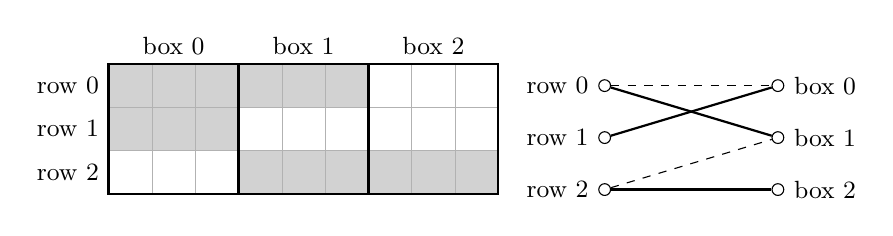
\begin{tikzpicture}[x=0.55cm,y=0.55cm]
  % a band: 3 rows x 9 columns; shaded mini-rows hold candidates for d
  \foreach \r/\k in {0/0,0/1,1/0,2/1,2/2} {
    \fill[gray!35] (3*\k,2-\r) rectangle (3*\k+3,3-\r);
  }
  \draw[step=1,gray!60,very thin] (0,0) grid (9,3);
  \draw[thick] (0,0) rectangle (9,3);
  \foreach \x in {3,6} \draw[thick] (\x,0) -- (\x,3);
  \foreach \r in {0,1,2} \node[left] at (0,2.5-\r) {\small row \r};
  \foreach \k in {0,1,2} \node[above] at (3*\k+1.5,3) {\small box \k};
  % bipartite graph
  \begin{scope}[xshift=6.3cm]
    \foreach \r in {0,1,2} \node[circle,draw,inner sep=1.5pt,label=left:{\small row \r}] (r\r) at (0,2.5-\r*1.2) {};
    \foreach \k in {0,1,2} \node[circle,draw,inner sep=1.5pt,label=right:{\small box \k}] (b\k) at (4,2.5-\k*1.2) {};
    \draw[thick] (r1) -- (b0);
    \draw[thick] (r0) -- (b1);
    \draw[thick] (r2) -- (b2);
    \draw[dashed] (r0) -- (b0);
    \draw[dashed] (r2) -- (b1);
  \end{scope}
\end{tikzpicture}
\caption{The band rule for one digit. Left: mini-rows of a band that still hold candidates for the digit. Right: the
bipartite graph of rows and boxes. Row 1 can only use box 0, which forces row 0 into box 1 and row 2 into box 2;
the dashed edges lie on no perfect matching, so the band rule removes the digit from mini-rows (0, 0) and (2, 1).
The stack rule is the same test on bands and the columns of a stack.}
\label{fig:band}
\end{figure}

The rule costs four table lookups: three 512-entry lookups turn the 27-bit band into the 9-bit matrix $A$, and a
512-entry table maps $A$ to the cells of the mini-rows that lie on a perfect matching. This is the core of the band
solvers of \cref{sec:background}; it covers the consequences of the digit's row and box constraints within the band (locked candidates between rows
and boxes), while placing a digit, and removing the other digits from its cell, is a separate step.

Transposing the argument gives the \textbf{stack rule}. Within a stack, $d$ occurs once in each of its three columns
and once in each of its three boxes, and the boxes of a stack correspond one-to-one to the bands. So $d$'s placement pairs the three bands one-to-one with the stack's three columns, and a (band,
column) pair can be kept only if it lies on a
perfect matching of the $3\times 3$ graph whose edges are the pairs where $d$ still has a candidate. The matrix is
read from each band's 9-bit set of columns in use, so the rule costs three table lookups per digit, and it only has
to run when some band's column set changes. It subsumes the locked-column step of JCZSolve, which removes a column
from the other bands when a box of this band has candidates in that column alone: that is the special case of a
band vertex with degree one. tdoku gets the same inference from its vertical triads.

\begin{proposition}[one kind of hidden single suffices]
Given the band and stack rules, hidden singles in rows imply those in boxes and columns at the fixed point of
propagation.
\end{proposition}
\begin{proof}[Argument]
If $d$ has one cell $c$ left in a box, the box's mini-row containing $c$ is the only edge at that box vertex, so the
band rule removes $d$ from the rest of $c$'s row, leaving $c$ as a row single. If $d$ has one cell $c$ left in a
column, that column is the only edge of the stack graph at the column vertex, so the stack rule removes $d$'s other
columns from $c$'s band within the stack; the box of $c$ is then down to the single cell $c$, and the band rule reduces $c$'s
row to $c$.
\end{proof}

Empirically, in a reference solver that applies every rule to every (digit, band) in each round, removing box and
column hidden singles from a solver with both rules and row singles leaves the search tree unchanged on the 1106
forum-hardest, 17-clue, magictour and kaggle sets (284.2 vs.\ 284.2 nodes per puzzle on 1106), but propagation takes
up to 6\% more rounds per node, because those singles are then found a round later (8.11 vs.\ 7.62 on 17-clue).
Dropping row singles too doubles the tree (621 nodes on 1106).

\section{FastBandSolver}
\label{sec:solver}

This section describes the implementation in enough detail to rebuild it; the code is a single C++20 header,
\texttt{fastbandsolver.hpp}, of about 400 lines. It solves one puzzle at a time on one thread.

\paragraph{Overview.} The solver keeps, for every digit and every band, a 27-bit mask of the cells where the digit can
still go (\cref{sec:state}). Solving a node of the search tree repeats three steps until nothing changes. (1) For each
mask that changed, apply the band rule, the stack rule and row singles (\cref{alg:band,alg:stack}); these are the
cheap, frequent steps, done with a few table lookups each. (2) Count, for each cell, how many digits it still admits,
using bitwise tricks that handle all 27 cells of a band at once; a cell with none means a dead end, a cell with one is
a naked single to place. (3) When nothing changes and cells remain open, guess: pick the two-candidate cell with the
most open cells around it, and try both digits (\cref{alg:search}). Everything else in this section is about doing
these steps with as few instructions and as few unpredictable branches as possible.

\subsection{State and bit layout}
\label{sec:state}

Following zhouyundong~\cite{zhouyundong2012solver}, candidates are stored by digit and band. For digit
$d\in\{0,\dots,8\}$ and band $b\in\{0,1,2\}$, the 32-bit word $M_{d,b}$ holds a 27-bit mask of the cells of band $b$
where $d$ can still go, with bit $9r+c$ for row $r\in\{0,1,2\}$ of the band and column $c\in\{0,\dots,8\}$:

\begin{center}
\small
\begin{tabular}{ccc}
bits 26\ldots18 & bits 17\ldots9 & bits 8\ldots0 \\
\midrule
row 2 (cols 8\ldots0) & row 1 (cols 8\ldots0) & row 0 (cols 8\ldots0) \\
\end{tabular}
\end{center}

\noindent Within each 9-bit row, bits $3k$, $3k{+}1$, $3k{+}2$ are the \emph{mini-row} of box $k$. We write masks in octal (base 8),
marked with a subscript 8: each octal digit is three bits, so a band mask is nine octal digits, one per mini-row,
read from row 2, box 2 on the left to row 0, box 0 on the right. For example $777_8 = 511$ is nine 1-bits, the mask
of one row. Two shifts, two ORs
and an AND give the band's \emph{column set} $P(M)=(M \mid M\gg 9 \mid M\gg 18)\ \&\ 777_8$, the columns where the digit still has a
candidate in the band, and $\mathrm{cols}(x)=x \mid x\ll 9 \mid x\ll 18$ spreads a 9-bit column set back to cells (two shifts
and two ORs).

The search state is a plain struct:

\begin{center}
\small
\begin{tabular}{lll}
\toprule
field & type & meaning \\
\midrule
\texttt{cells[27]} & 32-bit & $M_{d,b}$ at index $3d+b$ \\
\texttt{checked[27]} & 32-bit & $M_{d,b}$ as it was the last time the band rules ran on it (0 initially) \\
\texttt{unsolved[3]} & 32-bit & cells of each band not yet given a digit \\
\texttt{openRows[9]} & 16-bit & per digit, 9 bits: rows ($3b+r$) where the digit is not yet placed \\
\bottomrule
\end{tabular}
\end{center}

\noindent That is 246 bytes. A placed digit keeps its cell in $M_{d,b}$, so a solved grid is one in which every cell
has exactly one candidate. The solver owns an array of 82 states; the state for search depth $t$ is slot $t$, and a
guess copies slot $t$ into slot $t{+}1$ with one \texttt{memcpy} (a block copy of
memory). No memory is allocated during a solve.

\subsection{Lookup tables}

All tables are computed at compile time (\texttt{constexpr}) and total 8{,}548 bytes.

\begin{center}
\small
\begin{tabular}{llp{8.2cm}}
\toprule
table & entries & contents \\
\midrule
\texttt{BOXES\_OF\_ROW} & 512 $\times$ 8 bit & for a 9-bit row, the boxes (3 bits) it has candidates in \\
\texttt{MATCHABLE} & 512 $\times$ 16 bit & for a $3\times 3$ 0-1 matrix (bit $3i+j$), the union of the perfect matchings
  it contains, i.e.\ its entries that lie on some perfect matching. Built by testing the 6 permutations \\
\texttt{POSSIBLE\_CELLS} & 512 $\times$ 32 bit & for a mini-row matrix $A$ (bit $3r+k$), the band cells of the mini-rows
  in \texttt{MATCHABLE}$[A]$ \\
\texttt{ONE\_COLUMN\_BOXES} & 512 $\times$ 8 bit & for a band's column set, the boxes (3 bits) with exactly one column \\
\texttt{SINGLE\_ROWS} & 4096 $\times$ 8 bit & for \texttt{MATCHABLE}$[A]$ and \texttt{ONE\_COLUMN\_BOXES}$[P]\ll 9$, the rows
  (3 bits) down to one cell (\cref{lem:singlerows}) \\
\texttt{AFTER\_PLACING} & 27 $\times$ 32 bit & for a cell, the band minus the cell's row and box, plus the cell \\
\texttt{OTHER\_BANDS\ldots} & 27 $\times$ 32 bit & for a cell, all cells of a band except the cell's column \\
\texttt{BAND\_PEERS} & 27 $\times$ 32 bit & for a cell, its row and box within the band, the cell excluded \\
\texttt{ROWS\_CELLS} & 8 $\times$ 32 bit & for a 3-bit row set, the cells of those rows \\
\bottomrule
\end{tabular}
\end{center}

\subsection{The band update}

\Cref{alg:band} is the inner step, run on one (digit, band) mask. It is written as a C++ template on the band index, so the compiler generates a separate copy for each band in which
the positions of the two other bands are constants. It is also forced \emph{inline}: its code is copied into the update
loop instead of being called as a function, which avoids the cost of a call.

\begin{algorithm}[t]
\caption{\textsc{UpdateBand}$_b(S, d)$: band rule, stack rule and row singles for digit $d$ in band $b$}
\label{alg:band}
\begin{algorithmic}[1]
\State $M \gets S.\mathit{cells}[3d+b]$; \ $M_{\mathrm{old}} \gets S.\mathit{checked}[3d+b]$
\State $A \gets \textsc{BoxesOfRow}[M \,\&\, 777_8] \mid \textsc{BoxesOfRow}[(M\gg 9)\,\&\,777_8]\ll 3 \mid
  \textsc{BoxesOfRow}[M\gg 18]\ll 6$ \Comment{mini-row matrix}
\State $M \gets M \,\&\, \textsc{PossibleCells}[A]$ \Comment{band rule}
\If{$M = 0$} \Return \textbf{contradiction} \EndIf
\State $S.\mathit{cells}[3d+b] \gets M$; \ $S.\mathit{checked}[3d+b] \gets M$
\State $P \gets P(M)$
\If{$P \ne P(M_{\mathrm{old}})$} \textsc{StackRule}$(S, d)$ \EndIf
\State $R \gets \textsc{SingleRows}[\textsc{Matchable}[A] \mid \textsc{OneColumnBoxes}[P]\ll 9]$
\State $N \gets R \,\&\, (S.\mathit{openRows}[d] \gg 3b) \,\&\, 7$ \Comment{rows newly down to one cell}
\If{$N \ne 0$}
  \State $C \gets M \,\&\, \textsc{RowsCells}[N]$ \Comment{the placed cells, one per row}
  \For{$e \gets 0$ \textbf{to} $8$} $S.\mathit{cells}[3e+b] \gets S.\mathit{cells}[3e+b] \,\&\, \lnot C$ \EndFor
  \State $S.\mathit{cells}[3d+b] \gets M$ \Comment{restore $d$'s own cells}
  \State $S.\mathit{unsolved}[b] \gets S.\mathit{unsolved}[b] \,\&\, \lnot C$; \
    $S.\mathit{openRows}[d] \gets S.\mathit{openRows}[d] \,\&\, \lnot(N\ll 3b)$
\EndIf
\State \Return \textbf{ok}
\end{algorithmic}
\end{algorithm}

Line 2 turns the 27-bit mask into the $3\times 3$ mini-row matrix $A$ with three 512-entry lookups, one per row. Line 3
applies the band rule of \cref{sec:rules}: \textsc{PossibleCells}$[A]$ is the set of cells of mini-rows on some perfect
matching, so one AND removes every candidate of $d$ that no row-to-box arrangement can use. If no perfect matching
exists the table entry is 0 and the band is a contradiction (line 4). Lines 6--7 run the stack rule only when the
band's column set changed; because \texttt{checked} starts at 0, every band triggers it once on its first update. The
stack rule may shrink this band again; since \texttt{checked} keeps the value from line 5, the band then differs from
its checked value and is updated again in the next pass.

Lines 8--9 find the rows that are down to one cell without examining the rows bit by bit:

\begin{lemma}
\label{lem:singlerows}
After line 3, row $r$ of the band has exactly one candidate cell if and only if row $r$ has exactly one matchable box
$k$ and box $k$ has exactly one column in $P$.
\end{lemma}
\begin{proof}
After line 3 every remaining mini-row lies on a perfect matching, so row $r$ has candidates exactly in its matchable
boxes. If row $r$ has two matchable boxes it has at least two cells. If it has exactly one, $k$, then every perfect
matching sends $r$ to $k$, so no other row keeps a candidate in box $k$, and the candidates of box $k$ are those of
row $r$'s mini-row. That mini-row is one cell exactly when box $k$ has one column.
\end{proof}

\noindent So \textsc{SingleRows} is indexed by the 9-bit matchable matrix and the 3-bit set of one-column boxes, 4096
entries. Line 9 keeps only rows where $d$ is not yet placed, so each placement is made once. Placing row singles
(lines 10--15) clears the placed cells from all nine digits of the band in straight-line code and then restores $d$'s
own mask, which is cheaper than testing \texttt{other != digit} in the loop.

\paragraph{Worked example.} Let $d$ have candidates in columns $\{1,4\}$ of row 0, $\{0,2\}$ of row 1 and $\{3,8\}$
of row 2, the configuration of \cref{fig:band}. Then $M=410005022_8$. The row lookups give box sets $\{0,1\}$,
$\{0\}$ and $\{1,2\}$, so $A=110\,001\,011_2=395$. The only perfect matching is row 0 $\to$ box 1, row 1 $\to$ box 0,
row 2 $\to$ box 2, so \textsc{Matchable}$[395]=100\,001\,010_2=266$, and line 3 leaves columns $\{4\}$, $\{0,2\}$ and
$\{8\}$: $M=400005020_8$. The column set is $\{0,2,4,8\}$; box 0 has two columns and boxes 1 and 2 one each, so
\textsc{OneColumnBoxes}$=110_2$, and \textsc{SingleRows} returns rows $\{0,2\}$: $d$ is placed in row 0, column 4 and
row 2, column 8, and those two cells are removed from the other eight digits.

\subsection{The stack rule}

\begin{algorithm}[t]
\caption{\textsc{StackRule}$(S, d)$}
\label{alg:stack}
\begin{algorithmic}[1]
\State $p_b \gets P(S.\mathit{cells}[3d+b])$ for $b = 0,1,2$ \Comment{9-bit column sets}
\State $K_0, K_1, K_2 \gets 0$
\For{$s \gets 0, 3, 6$} \Comment{the three stacks}
  \State $m \gets (p_0\gg s \,\&\, 7) \mid (p_1\gg s \,\&\, 7)\ll 3 \mid (p_2\gg s \,\&\, 7)\ll 6$ \Comment{bands $\times$ columns}
  \State $o \gets \textsc{Matchable}[m]$
  \State $K_b \gets K_b \mid ((o \gg 3b)\,\&\,7)\ll s$ for $b = 0,1,2$
\EndFor
\State $S.\mathit{cells}[3d+b] \gets S.\mathit{cells}[3d+b] \,\&\, \mathrm{cols}(K_b)$ for $b = 0,1,2$
\end{algorithmic}
\end{algorithm}

\Cref{alg:stack} builds, for each stack, the $3\times 3$ matrix of bands by the stack's three columns and keeps the
pairs on some perfect matching, reusing \textsc{Matchable}. It is branch-free: three lookups and a few dozen shifts,
ANDs and ORs. For example, if in stack 0 the digit's columns are $\{0,1\}$ in band 0, $\{0\}$ in band 1 and
$\{0,1,2\}$ in band 2, the matching forces band 1 $\to$ column 0, band 0 $\to$ column 1 and band 2 $\to$ column 2, and
the rule removes three of the six pairs present. The locked-column step of JCZSolve is the case where a band has one column
in a stack; we removed it, as the stack rule covers it and runs only when column sets change. Processing only the
stacks whose columns changed produced the same tree but was 19\% slower, because the per-stack branches mispredict.

\subsection{The update loop and propagation}

\begin{algorithm}[t]
\caption{\textsc{Update}$(S)$ and \textsc{Propagate}$(S)$}
\label{alg:propagate}
\begin{algorithmic}[1]
\Function{Update}{$S$}
  \Repeat
    \State $\mathit{again} \gets \mathbf{false}$
    \For{$d \gets 0$ \textbf{to} $8$}
      \For{$b \gets 0$ \textbf{to} $2$} \Comment{unrolled}
        \If{$S.\mathit{cells}[3d+b] \ne S.\mathit{checked}[3d+b]$}
          \If{\textsc{UpdateBand}$_b(S,d)$ fails} \Return \textbf{contradiction} \EndIf
          \State $\mathit{again} \gets \mathbf{true}$
        \EndIf
      \EndFor
    \EndFor
  \Until{\textbf{not} $\mathit{again}$}
\EndFunction
\Function{Propagate}{$S$}
  \Loop
    \If{\textsc{Update}$(S)$ fails} \Return \textbf{contradiction} \EndIf
    \State $\mathit{placed} \gets \mathbf{false}$; \ $\mathit{multi} \gets 0$
    \For{$b \gets 0$ \textbf{to} $2$}
      \State $u_1, u_2, u_3 \gets 0$
      \For{$d \gets 0$ \textbf{to} $8$} \Comment{bit-sliced counters, saturating at 3}
        \State $u_3 \gets u_3 \mid (u_2 \,\&\, M_{d,b})$; \ $u_2 \gets u_2 \mid (u_1 \,\&\, M_{d,b})$; \ $u_1 \gets u_1 \mid M_{d,b}$
      \EndFor
      \If{$u_1 \ne 2^{27}-1$} \Return \textbf{contradiction} \Comment{a cell with no candidate} \EndIf
      \State $\mathit{pairs}_b \gets u_2 \,\&\, \lnot u_3$; \ $\mathit{multi} \gets \mathit{multi} \mid u_2$
      \For{each cell $x$ in $u_1 \,\&\, \lnot u_2 \,\&\, S.\mathit{unsolved}[b]$} \Comment{naked singles}
        \State $d \gets$ the digit with $x \in M_{d,b}$; \textbf{if} none \Return \textbf{contradiction}
        \State \textsc{PlaceNaked}$(S, d, b, x)$; \ $\mathit{placed} \gets \mathbf{true}$
      \EndFor
    \EndFor
    \If{\textbf{not} $\mathit{placed}$}
      \State \Return ($\mathit{multi} = 0$ ? \textbf{solved} : \textbf{open})
    \EndIf
  \EndLoop
\EndFunction
\end{algorithmic}
\end{algorithm}

\textsc{Update} (\cref{alg:propagate}) scans the 27 masks in digit order and runs \textsc{UpdateBand} on each one that
changed, until a pass changes nothing. Changes made during a pass (by the stack rule, or by row singles clearing cells
of other digits) are picked up later in the same pass or in the next one; the order does not affect the fixed point,
because every rule only removes candidates, and removing a candidate never makes a later removal wrong
(the rules are \emph{monotone}), so any order of applying them reaches the same end state.

\textsc{Propagate} then counts, for each band, how many digits each cell still admits. The three words
$u_1,u_2,u_3$ are bit-sliced saturating counters: bit $x$ of $u_i$ is set when at least $i$ digits admit cell $x$, so
27 cells are counted with five operations per digit (two ANDs and three ORs, all 27 cells at once). A cell in no digit's mask is a contradiction; cells with exactly
two candidates ($u_2\,\&\,\lnot u_3$) are the branching candidates; cells with one candidate that are not yet marked
solved are naked singles. A naked single of digit $d$ at cell $x$ is placed by \textsc{PlaceNaked}: $M_{d,b}$ is ANDed
with \textsc{AfterPlacing}$[x]$ (removing $d$ from the rest of $x$'s row and box), the other two bands of $d$ are ANDed
with \textsc{OtherBands}$[x]$ (removing $d$ from $x$'s column), $x$ is cleared from \texttt{unsolved}, and $x$'s row
is cleared from $d$'s \texttt{openRows}. The other digits need no work, because $x$ is not in their masks. If any
naked single was placed, the loop repeats; otherwise \textsc{Propagate} returns \emph{solved} when no cell has two or
more candidates, and \emph{open} with the two-candidate cells otherwise.

\subsection{Search and branching}

\begin{algorithm}[t]
\caption{\textsc{Search}$(S_t)$ at depth $t$}
\label{alg:search}
\begin{algorithmic}[1]
\State $r \gets \textsc{Propagate}(S_t)$
\If{$r = $ \textbf{contradiction}} \Return \EndIf
\If{$r = $ \textbf{solved}} record the solution; \Return \EndIf
\State $x \gets \arg\max_{x \in \mathit{pairs}} \textsc{PeerScore}(x)$, first in (band, bit) order among ties
\If{$x$ exists}
  \State $d_1 < d_2 \gets$ the two candidates of $x$
  \State $S_{t+1} \gets S_t$; \ \textsc{Place}$(S_{t+1}, d_1, x)$; \ \textsc{Search}$(S_{t+1})$
  \If{fewer than $\mathit{limit}$ solutions found} \textsc{Place}$(S_t, d_2, x)$; \ \textsc{Search}$(S_t)$ \EndIf
\Else
  \State $x \gets$ an unsolved cell with the fewest candidates, highest \textsc{PeerScore} among ties
  \For{each candidate $d$ of $x$, while fewer than $\mathit{limit}$ solutions found}
    \State $S_{t+1} \gets S_t$; \ \textsc{Place}$(S_{t+1}, d, x)$; \ \textsc{Search}$(S_{t+1})$
  \EndFor
\EndIf
\end{algorithmic}
\end{algorithm}

\Cref{alg:search} is a depth-first search that stops once \emph{limit} solutions are found; with limit 2 on a puzzle
with one solution it explores the whole tree. The second child of a two-candidate branch reuses the parent's slot,
since the parent is not needed afterwards. \textsc{Place} is the full placement used for guesses and clues: it removes
the cell from all nine digits, restores it in $d$'s mask, then does what \textsc{PlaceNaked} does.

\textsc{PeerScore}$(x)$ for cell $x$ at index $i$ of band $b$ counts the unsolved cells among $x$'s 20 peers:
\[
\mathrm{popcount}\bigl(U_b \,\&\, \textsc{BandPeers}[i]\bigr) + \mathrm{popcount}\bigl((U_{b'} \,\&\, \mathrm{col}_i) \mid
(U_{b''} \,\&\, \mathrm{col}_i)\ll 32\bigr),
\]
where $U$ are the \texttt{unsolved} masks, $b'$, $b''$ the other bands and $\mathrm{col}_i$ the three cells of $x$'s
column in a band; packing the two other bands into one 64-bit word makes it two popcounts. At branch time, after
propagation, the unsolved cells are exactly the cells with two or more candidates, so the score is the number of
peers still open. We count one guess per two-candidate branch and $n-1$ for an $n$-candidate fallback cell, the
number of binary decisions the branch represents.

\textsc{Load} starts from all candidates, \texttt{checked} at 0 and all rows open, and places each clue with
\textsc{Place} after checking that the clue is still a candidate; a repeated clue in a row, column or box fails that
check and the puzzle has no solution. Clues are only placed, not propagated: the first \textsc{Propagate} does that.

\subsection{Correctness}

\begin{proposition}
\textup{\textsc{Search}} returns the number of solutions, up to the limit, and a valid first solution.
\end{proposition}
\begin{proof}[Argument]
\emph{Soundness}: each elimination removes a candidate that no solution extending the current candidates can use
(the band and stack rules by \cref{sec:rules}; row and naked singles and placement by the Sudoku constraints), and a
contradiction is reported only when a band has no arrangement or a cell no candidate, so no solution is lost.
\emph{Completeness of branching}: the children of a branch partition the candidates of one cell. \emph{Solved
states}: \textsc{Propagate} returns \emph{solved} only after an \textsc{Update} fixed point with no naked single left
and every cell at exactly one candidate. At the fixed point every band mask has passed the band rule, so each digit
has a candidate in every row and box of every band; and the stack rule ran after the last change to each band's
column set, so each digit has a candidate in every column. With one digit per cell and nine cells per unit, each
digit is then in each row, column and box exactly once, so the grid is a solution. It is recorded once, because the
children of each branch are disjoint.
\end{proof}

The \texttt{checked} masks make the fixed point cheap to detect but must be handled with care, and we hit three bugs
worth recording for anyone reimplementing this. (1) Returning \emph{solved} as soon as \texttt{unsolved} is empty,
before counting candidates, accepted grids in which a placement had emptied an earlier cell. (2) An update loop that
skips digits with no open rows, as JCZSolve's does, never re-checks such a digit; our first version relied on that
update to clear a placed digit's column, and recorded grids with a digit twice in a column. We now clear the column
at placement time and do not skip digits. (3) Two naked singles in one band can conflict, so the search for the
single's digit must be bounded. Bugs (1) and (2) showed only on the 1905 set, as a second ``solution'' of 5 to 7
unique puzzles; bug (3) only under AddressSanitizer (a compiler option that reports
out-of-bounds memory accesses) on puzzles with many solutions. Our correctness checks compare
solution counts with tdoku and with a naive counter, and validate every solution.

\subsection{Work profile}

\Cref{tab:work} counts what the solver does per puzzle. On the hardest set it propagates 275 times per puzzle (136
branch nodes, each with up to two children); each propagation runs \textsc{UpdateBand} about 12 times, in 3.3 passes of the update
loop. Placements come almost entirely from row singles (1{,}920 per puzzle) rather than naked
singles (84), because the solver detects hidden singles only in rows; the matching rules turn box and column
singles into row singles (\cref{sec:rules}). The stack rule runs on 70\% of band
updates but changes something on only 41\% of its calls. Dividing the instruction count of \cref{tab:counters} by the
band updates gives about 176 instructions per band update on the hardest set, everything included.

\begin{table}[t]
\centering
\caption{Work per puzzle, limit 2.}
\label{tab:work}
\small
\begin{tabular}{lrrr}
\toprule
& forum hardest 1106 & 17 clue & kaggle \\
\midrule
\textsc{Propagate} calls & 274.8 & 2.3 & 1.0 \\
\textsc{Update} passes & 901.2 & 15.7 & 3.6 \\
\textsc{UpdateBand} calls & 3360.8 & 117.7 & 36.8 \\
\textsc{StackRule} calls (that changed a mask) & 2362.1 (962.3) & 93.3 (32.0) & 36.0 (11.2) \\
row singles placed & 1919.7 & 70.2 & 47.2 \\
naked singles placed & 84.4 & 1.2 & 0.0 \\
branch nodes (fallback nodes) & 136.1 (1.55) & 0.7 (0.00) & 0.0 \\
guesses & 137.7 & 0.7 & 0.0 \\
\bottomrule
\end{tabular}
\end{table}

\subsection{Engineering}

We measured each change by alternating builds and taking medians (\cref{sec:setup}). Four details each moved the time
by 3\% or more on the hard sets. Forcing \textsc{UpdateBand} to be inlined saved 9\%: clang otherwise emitted a call
for each band update. The table-driven row singles of \cref{lem:singlerows} saved 5.6\% over per-row bit arithmetic.
Not skipping digits whose rows are all placed saved 4\%. Replacing locked columns entirely by the stack rule saved 3\%.
Three changes that looked promising were slower and were dropped: processing only the stacks that changed (19\%
slower), batching the stack rule once per digit per pass (14\% slower, because eliminations applied immediately help
the rest of the pass), and forcing the stack rule inline (1\% slower).

\section{Experimental setup}
\label{sec:setup}

All measurements are on an Apple M4 Max (14 cores, 36\,GB), macOS 15.6, Apple clang 17.0.0 with \texttt{-O3
-march=native}, single-threaded. We use tdoku's five standard data sets~\cite{dillon2019nerdsniped}: the 49{,}158
known 17-clue puzzles~\cite{royle17clue,champagne2022all17}, magictour's top 1465~\cite{stertenbrink2005top1465}, the forum-hardest collections (375
puzzles from ``1106''\footnote{tdoku's documentation describes this set as 376 puzzles; its data file holds 375.} and
48{,}766 from ``1905\_11+'')~\cite{forumhardest}, and 100{,}000 puzzles from the Kaggle
data set~\cite{park2016kaggle}. Following tdoku's benchmarks, every solver is called with a solution limit of 2, so it
must show uniqueness, and converting the puzzle string is part of each call. Before timing, each solver must solve
every puzzle with a valid solution and agree with the others on the number of solutions. Solvers take turns over the
whole data set, and we report the median of seven runs. tdoku is built from our ARM port~\cite{kelly2026tdokuarm}, described in \cref{sec:arm}. \texttt{make sota} in the repository reproduces \cref{tab:sota} for every solver but JCZSolve (see below), to two significant figures.

\subsection{ARM and x86}
\label{sec:arm}

\paragraph{Why the processor family matters.} Almost all published Sudoku benchmarks, including tdoku's, were run on
x86 processors from Intel and AMD. Our machine is an Apple M4 Max, whose cores use the 64-bit ARM instruction set
(AArch64). The two families differ in the SIMD instructions they offer (\cref{sec:terms}). x86 has 128-bit SSE, 256-bit
AVX2 and, on some Intel processors, 512-bit AVX-512, with a rich set of byte-shuffle and bit-counting instructions.
AArch64 has 128-bit NEON, whose instructions overlap with SSE's but are not the same. Code written with x86 SIMD
\emph{intrinsics} (C functions that map one-to-one onto SIMD instructions, such as \texttt{\_mm\_shuffle\_epi8}) does
not compile on ARM at all. Plain C and C++ code, by contrast, compiles for either family, and the compiler chooses the
instructions.

\paragraph{The solvers that needed no porting.} FastBandSolver, JCZSolve, jsolve and kudoku are plain C or C++ with
no SIMD intrinsics. They use 32- or 64-bit integer operations, small lookup tables, and, in FastBandSolver's case,
\texttt{std::popcount}, which compiles to a hardware bit-count on both families. We built them unchanged with Apple
clang and \texttt{-O3 -march=native}. The same source files build on x86; we did not have an x86 machine to measure
them on.

\paragraph{Porting tdoku.} tdoku is written against x86 intrinsics and did not build on ARM: its SIMD header includes
the x86-only \texttt{immintrin.h}. All of its SIMD code goes through two small vector classes: \texttt{Bitvec08x16},
eight 16-bit lanes in a 128-bit register, and \texttt{Bitvec16x16}, sixteen lanes in 256 bits. The only ARM build we
found translated the x86 intrinsics with the SIMDe library, and because compilers for ARM do not define x86 feature macros such as \texttt{\_\_SSE4\_1\_\_}, tdoku's
own preprocessor checks sent that build down its slowest code path, written for 2000-era SSE2. Our port~\cite{kelly2026tdokuarm}
adds a native NEON implementation of \texttt{Bitvec08x16} in which every method reproduces the behavior of tdoku's
SSSE3/SSE4 code path exactly, including details such as how a byte shuffle treats out-of-range indices and which lane
wins a tie in a minimum search. \texttt{Bitvec16x16} becomes a pair of 128-bit halves, as tdoku already does on x86
processors without AVX2. The solver itself is unchanged, and the x86 build is unaffected: the preprocessed header is
byte-identical for every x86 instruction set tdoku supports. We verified the port three ways. (1) Against real x86
tdoku: the unmodified x86 build, run on the M4 through Apple's Rosetta 2 translator, and the native ARM build return
the same solution counts, solutions and guess counts on all 199{,}807 puzzles of tdoku's test and benchmark sets. (2)
Method by method: the NEON class and the original SSE4.1 code (built on ARM through SIMDe) agree on 62.9 million
random and edge-case inputs, and the test detects each of three deliberately planted bugs. (3) Sanitizers report
no errors. \Cref{tab:port} shows what the port is worth: native NEON is 1.3 times faster than the SSE4.1 path through
SIMDe and about 3 times faster than the SSE2 path, and 1.23 times faster than the x86 build under Rosetta.

\begin{table}[t]
\centering
\caption{tdoku on the M4 Max, \si{\micro\second} per puzzle, limit 2, under three ways of running its x86 SIMD code on
ARM~\cite{kelly2026tdokuarm}.}
\label{tab:port}
\small
\begin{tabular}{lrrr}
\toprule
data set & native NEON (our port) & SIMDe, SSE4.1 path & SIMDe, SSE2 path \\
\midrule
17 clue & 2.89 & 3.68 & 8.54 \\
magictour top 1465 & 8.04 & 10.71 & 24.00 \\
forum hardest 1106 & 72.4 & 94.9 & 219.9 \\
\bottomrule
\end{tabular}
\end{table}

\paragraph{What the port cannot recover.} NEON registers are 128 bits wide, so on the M4 tdoku runs its 256-bit
operations as two 128-bit ones, as on x86 without AVX2; the fastest published tdoku results use AVX2 or AVX-512.


\section{Results}
\label{sec:results}

\begin{table}[t]
\centering
\caption{Time per puzzle in \si{\micro\second} (guesses per puzzle), limit 2, median of 7 interleaved runs, Apple M4 Max.
Every solver solves every puzzle with a valid solution and agrees on the solution counts. Guesses are each solver's
own count of binary decisions.}
\label{tab:sota}
\small
\setlength{\tabcolsep}{4pt}
\begin{tabular}{lrrrrrr}
\toprule
data set & puzzles & FastBandSolver & tdoku & JCZSolve & jsolve & kudoku \\
\midrule
17 clue & 49158 & \textbf{1.83} (0.68) & 2.96 (0.57) & 2.48 (2.37) & 3.04 (0.60) & 15.0 (4.51) \\
magictour top 1465 & 1465 & \textbf{7.00} (10.3) & 8.44 (8.94) & 10.2 (22.0) & 13.0 (12.1) & 65.8 (33.9) \\
forum hardest 1106 & 375 & \textbf{62.6} (138) & 75.1 (110) & 109 (363) & 151 (183) & 573 (326) \\
forum hardest 1905 11+ & 48766 & \textbf{39.7} (81.0) & 46.8 (61.7) & 56.3 (167) & 91.2 (100) & 275 (142) \\
kaggle & 100000 & \textbf{0.866} (0) & 0.936 (0) & 1.21 (0) & 1.56 (0) & 7.57 (0) \\
\bottomrule
\end{tabular}
\end{table}

\Cref{tab:sota} compares FastBandSolver with tdoku and with the fastest cell-based (jsolve), band-based (JCZSolve)
and exact-cover (kudoku) solvers from tdoku's benchmark. FastBandSolver is fastest on every set: 1.20$\times$ faster
than tdoku on the 375 hardest puzzles, 1.18$\times$ on the 48{,}766 of the second forum set, 1.21$\times$ on
magictour, 1.62$\times$ on 17-clue and 1.08$\times$ on kaggle. JCZSolve is not part of \texttt{make sota} because its
source leaves the copyright unspecified;\footnote{In a 2018 forum thread its three contributors agreed to its use in
rust\_sudoku: zhouyundong\_2012 without conditions, JasonLion under AGPLv3, and champagne for free use. We did not
treat this as a license for redistribution.} we built it from tdoku's copy for local measurement only.

tdoku still makes the fewest guesses: its triad propagation and configuration branching leave a 20\% smaller tree
than ours on the hardest set. FastBandSolver wins on cost per node. Hardware counters (\cref{tab:counters}) show it
retiring 23\% fewer instructions than tdoku per hard puzzle at a slightly lower IPC.

\begin{table}[t]
\centering
\caption{Instructions and cycles per puzzle, limit 2, from the processor's counters.}
\label{tab:counters}
\begin{tabular}{llrrr}
\toprule
data set & solver & instructions & cycles & IPC \\
\midrule
forum hardest 1106 & FastBandSolver & 591{,}446 & 250{,}975 & 2.36 \\
 & tdoku & 768{,}634 & 298{,}921 & 2.57 \\
 & JCZSolve & 936{,}136 & 434{,}561 & 2.15 \\
\midrule
17 clue & FastBandSolver & 18{,}866 & 7{,}634 & 2.47 \\
 & tdoku & 34{,}121 & 12{,}139 & 2.81 \\
 & JCZSolve & 18{,}289 & 10{,}225 & 1.79 \\
\bottomrule
\end{tabular}
\end{table}

\paragraph{Ablation.} \Cref{tab:ablation} switches the three changes of \cref{sec:solver} on and off in the same
engine. With all three off the search is JCZSolve's (361 vs.\ 363 guesses on the hardest set), and the engine is
about 10\% slower than JCZSolve per node. Peer-count branching is the largest single effect: it removes 45\% of the
guesses on the hardest set and 28\% of the time. The stack rule removes another 20\% of the guesses. The fallback
fires at only 1.1\% of branch nodes on the hardest set, yet choosing a fewest-candidates cell there instead of the
first unsolved one removes 12\% of the guesses and 12\% of the time: these nodes tend to be near the root, and a
first unsolved cell often has five or more candidates. Of that gain, 3\% of the time comes from the peer-count tie
break. On the easy sets the stack rule costs 4--7\%: kaggle puzzles need no guesses, and there the extra
lookups are pure overhead.

\begin{table}[t]
\centering
\caption{Ablation: time per puzzle in \si{\micro\second} (guesses per puzzle), limit 2. Each variant is a separate
build of the same code; variants ran one after another, each taking the median of 5 runs per data set, and we report
the better of two such sweeps.}
\label{tab:ablation}
\small
\begin{tabular}{cccrrrrr}
\toprule
peer & stack & fewest & hardest 1106 & hardest 1905 & magictour & 17 clue & kaggle \\
branching & rule & fallback & & & & & \\
\midrule
 & & & 120.4 (361) & 61.7 (166) & 10.5 (22.0) & 2.16 (2.4) & 0.81 \\
 & & \checkmark & 105.0 (305) & 58.6 (155) & 10.4 (21.7) & 2.04 (1.9) & 0.81 \\
 & \checkmark & & 110.4 (315) & 55.5 (144) & 9.8 (18.8) & 2.07 (1.4) & 0.86 \\
 & \checkmark & \checkmark & 94.6 (262) & 52.3 (133) & 9.7 (18.5) & 2.01 (1.2) & 0.86 \\
\checkmark & & & 86.5 (197) & 49.4 (105) & 7.5 (12.3) & 1.84 (1.1) & 0.81 \\
\checkmark & & \checkmark & 76.6 (173) & 46.9 (99) & 7.5 (12.1) & 1.77 (0.9) & 0.81 \\
\checkmark & \checkmark & & 71.5 (157) & 42.0 (86) & 7.1 (10.4) & 1.89 (0.8) & 0.86 \\
\checkmark & \checkmark & \checkmark & \textbf{62.7} (138) & \textbf{39.8} (81) & \textbf{7.0} (10.2) & 1.84 (0.7) & 0.87 \\
\bottomrule
\end{tabular}
\end{table}

\paragraph{ARM compared with published x86 results.} We could not run the solvers on x86 ourselves, but tdoku's
repository publishes results for the same data sets on several x86 machines. \Cref{tab:x86} compares its results for
an Intel Core i7-1065G7 (a 2019 laptop processor with AVX-512, the machine our pull request compares against)
with ours. Two patterns stand out. The scalar solvers run 1.3--1.7 times faster on the M4 Max than on the Intel
processor, while tdoku runs 10--16\% slower. As a result tdoku's lead over JCZSolve, the scalar solver closest to ours,
shrinks from 1.3--2.5 times on the Intel processor to 0.84--1.45 times on the M4. These comparisons need care: they
are different machines, the published figures come from tdoku's own benchmark program (which times a random sample of
each data set), and each published figure is the best over a dozen compiler configurations, including profile-guided
optimization, while ours use one compiler. As a check on the harness, tdoku's own benchmark program on the M4 gives
13{,}446 puzzles per second on the hardest set~\cite{kelly2026tdokuarm}, and our harness 13{,}321.

\begin{table}[t]
\centering
\caption{The M4 Max against tdoku's published results for an Intel Core i7-1065G7 (best of all compiler configurations
per cell). Left: how much faster tdoku is than JCZSolve on each machine. Middle: speed on the M4 divided by speed on the
Intel processor. Right: FastBandSolver's measured speedup over tdoku on the M4, and a projection for the Intel
processor assuming FastBandSolver gains from the M4 as JCZSolve does.}
\label{tab:x86}
\small
\setlength{\tabcolsep}{4pt}
\begin{tabular}{lrrrrrrrr}
\toprule
& \multicolumn{2}{c}{tdoku / JCZSolve} & \multicolumn{4}{c}{M4 speed / Intel speed} & \multicolumn{2}{c}{FastBandSolver / tdoku} \\
\cmidrule(lr){2-3} \cmidrule(lr){4-7} \cmidrule(lr){8-9}
data set & Intel & M4 & tdoku & JCZSolve & jsolve & kudoku & M4 & Intel (projected) \\
\midrule
kaggle & 2.07 & 1.29 & 0.90 & 1.45 & 1.38 & 1.28 & 1.08 & 0.67 \\
17 clue & 1.33 & 0.84 & 0.90 & 1.43 & 1.66 & 1.49 & 1.62 & 1.02 \\
magictour top 1465 & 1.89 & 1.21 & 0.84 & 1.32 & 1.49 & 1.39 & 1.21 & 0.77 \\
forum hardest 1905 11+ & 2.01 & 1.20 & 0.87 & 1.46 & 1.47 & 1.41 & 1.18 & 0.71 \\
forum hardest 1106 & 2.45 & 1.45 & 0.85 & 1.44 & 1.49 & 1.36 & 1.20 & 0.71 \\
\bottomrule
\end{tabular}
\end{table}

The last column shows what this implies. FastBandSolver's engine is JCZSolve's design with a smaller search tree, so
its speed should depend on the processor much as JCZSolve's does. If it does, FastBandSolver would be about 0.7 times
tdoku's speed on the hard sets on that Intel processor, and about even on 17-clue: its advantage is a property of the
M4, not a general one. The smaller search tree would carry over, since it does not depend on the machine, but on a
processor where tdoku's wide SIMD pays off, it is not enough to make up the difference. Measuring FastBandSolver on
x86 is the most important piece of follow-up work.

\section{What did not work}
\label{sec:negative}

We tried five other directions before the design above. Each was measured on the hardest set against tdoku's
75\us{} and 110 guesses; we report them because each is a natural idea and none paid off here.

\paragraph{Template search.} The template or pattern-overlay method~\cite{stuart2008pom} treats each digit's placements as one
of 46{,}656 templates; complete per-digit inference means keeping only templates consistent with the candidates. After
band propagation, a hard puzzle has a median of 491 templates over all nine digits (90th percentile 787), few enough
to filter as 128-bit masks. But even removing every template that conflicts with the
candidates (generalized arc consistency), adding a rule that every cell must be covered by some digit's remaining
templates, and branching on cells, still makes 98 decisions per puzzle, and adding pairwise digit consistency gives 81: little
better than tdoku's 110, at a much higher cost per node. The forum-hardest puzzles are selected to resist
single-digit techniques, and complete single-digit inference does not collapse their trees.

\paragraph{Search-tree nodes in SIMD lanes.} With a limit of 2 on a puzzle with one solution, the whole tree must be
searched, so the order of nodes does not matter and several nodes can be propagated at once. We wrote a branch-free
propagation round that runs one board per 32-bit lane of NEON registers, and verified it inside a one-board search
against tdoku on all five sets; we did not build the scheduler that keeps the lanes full. One round costs 74\,ns per
board with 4 lanes (3{,}344 instructions per round for 4 boards, IPC 2.8), 62\,ns with 8 and 50\,ns with 16, and a
node needs 3.9 rounds to reach a fixed point; capping the rounds grows the tree faster than it saves work (1{,}340
board-rounds per puzzle at two rounds per node vs.\ 1{,}119 at the fixed point). That projects to 240--290\,ns per
node with 4--8 lanes, above the roughly 220\,ns per node of JCZSolve's incremental engine under the same peer-count
branching, and 195\,ns with 16 lanes, near parity before any scheduling cost. We stopped there: a frontier of 16 nodes
cannot be kept full over most of a tree of a few hundred nodes. Two things are missing: NEON has no gather, so the $3\times 3$ matching takes about 40 bit
operations instead of one lookup in a 512-entry table, and full rounds recompute all 27 (digit, band) masks where an
incremental engine touches only the changed ones.

\paragraph{Lookahead.} Probing both children of the best-scored two-candidate cells before branching, and taking a
failed probe as a free deduction, shrinks the tree fourfold: with JCZSolve's engine and 2 probed cells per node the
guesses fall from 199 to 49 on the hardest set. The time rises from 87 to 102\us, and probing only near the root, at
any threshold we tried, was never faster than not probing. In a slower reference solver the tree fell further (18
guesses with 64 probed cells), but at 1{,}282 probes per puzzle.

\paragraph{Richer rules and branching.} Triad rules for mini-rows and mini-columns (a mini-row whose cells admit exactly
three digits must hold all three, and three digits forced into a mini-row exclude the others) reduced the tree by
6--10\%, not enough to pay for themselves. Scoring bivalue cells and bilocations (a digit with two places left in a
unit) by the candidates they touch reduced the tree by another 18\% in the reference solver (121 vs.\ 148 guesses),
but computing the score cost about 0.9\us{} per branch node in a band solver, more than it saved. Scoring by the peer
candidates of the cell's two digits saves 1.5\% of guesses and costs 17\% of time. Branching on band configurations
as tdoku does was worse than peer-count branching with our rules (169 vs.\ 142 guesses).

\paragraph{Band decomposition.} A solution is three band fillings whose columns use disjoint digits, so solutions can
be counted by joining lists of band fillings, as in the enumeration of grids~\cite{felgenhauer2006mathematics}. After
propagation, however, the band with the fewest fillings still has a median of 888 of them on the hardest set (2{,}054
for the middle band), so the join alone is millions of pairs.

\section{Discussion}

The result depends on the machine (\cref{tab:x86}). On the M4 Max, scalar solvers with small, cache-resident tables
run 1.3--1.7 times faster than on a recent Intel processor, while tdoku runs slower, partly because NEON registers are
128 bits wide, so tdoku's 256-bit vectors become pairs of 128-bit operations, as on x86 without AVX2. All three solvers in \cref{tab:counters} run at an IPC between 2.1 and 2.6, and their
times follow their instruction counts and tree sizes. In that regime cheap choices of where to branch pay off more
than stronger propagation.

\paragraph{Limitations.} All measurements are from one machine and one compiler. We have not measured FastBandSolver on
x86, where tdoku can use AVX2 or AVX-512 and was designed to run; the projection of \cref{tab:x86} suggests it would
be slower than tdoku there on all but the 17-clue set. The data sets are those of tdoku's benchmark, and the forum-hardest sets are selected for difficulty
under human techniques, not under search. Guess counts are not directly comparable across solvers that branch on
different objects, which is why we compare times.

\section{Conclusion}

A scalar band solver with a matching-based stack rule, peer-count branching and a fewest-candidates fallback is faster than tdoku on all of tdoku's standard data sets on Apple Silicon, by 1.08--1.62$\times$. Branching carries most of the
gain. The advantage depends on the processor: on the M4 scalar code gains more than tdoku's SIMD code does, and a
projection from published results puts FastBandSolver at about 0.7 times tdoku's speed on a recent Intel processor
with AVX-512. Measuring it on x86 is the next step. The code and the benchmark are in the repository, and \texttt{make sota} reproduces \cref{tab:sota}.

\paragraph{Acknowledgments.} FastBandSolver's representation follows zhouyundong's band solver and its implementations
in JCZSolve and rust\_sudoku; the benchmark harness and data sets are Tom Dillon's. This work was done depending heavily on Anthropic's LLM harness Claude (Claude Code), using the model Claude Opus~5.5 with occasional advisory support from Claude Fable, including in theorizing, experimentation, and writeup.

\bibliographystyle{plain}
\bibliography{refs}

\end{document}
